\documentclass[a4paper,12pt]{article}

\usepackage{amsmath,amssymb,amsthm,tikz}
\usetikzlibrary{calc,arrows.meta}
\usepackage[margin=20mm]{geometry}
\usepackage{hyperref}
\usepackage{xcolor}
\usepackage{csquotes}

\setlength{\parindent}{0pt}
\setlength{\columnsep}{1cm}

\begin{document}

%\twocolumn

\thispagestyle{empty}

\begin{center}
{\Large Assignment 10: Red-Black Trees}
{\Large Published on 2020-11-25,}\\
{\em 12 minutes (estimated)} 
\end{center}

\noindent

{\bf TODO \#1.} Insert vertices that do not overlap with existing ones.\\
{\bf TODO \#2.} Ask to indicate the red/black vertices in the submitted answers.

A tree is named {\em Binary Search Tree} if the nodes satisfy the {\em order invariant}:
{\em Let $x$ be a node in a binary search tree. If $y$ is a node in the left subtree
of $x$, then $y.key \leq x.key$. If $z$ is a node in the right subtree of $x$, then
$z.key \geq z.key$.}

\vspace{10pt} A tree is named {\em Red-Black Tree}, if it is a Binary Search Tree, 
every node is either red or black (extra boolean flag stores this) and 
it satisfies these {\em red-black invariants}:
\begin{description}
\item[Root property] \hfill \\ The root is black.
\item[External property] \hfill \\ Every leaf (empty node) is also black.
\item[Internal property] \hfill \\  If a node is red, then both its children are black.
\item[Depth property] \hfill \\ For each node, all simple paths from the node to descendant leaves contain the
same number of black nodes. (See Figure~\ref{fig:original-tree}; leaves with NIL keys have 
black-height equal to $0$. As we move to the root, we increment 
the black-height $h_\text{black}$ whenever the path crosses some black node. 
The Depth property guarantees that each internal node gets the same black-height, no matter
which path from a leaf to a root we choose.)

\end{description}


{\em Note.} We call these tree properties {\em invariants}, because they should not change. 
For example, if there is any algorithm (inserting, deleting, rotating, etc.) on a {\em Binary Search Tree}
(and the original tree satisfies the order invariant), then after the manipulation the new 
Binary Search tree should also satisfy the order invariant.
We do not guarantee anything, if somebody gives a broken input (it is most likely 
``garbage-in, garbage-out'').\\
Same reasoning applies to the Red-Black Trees: If the original tree is red-black, then 
any manipulation should preserve the invariants (1),(2),(3),(4).



\begin{figure}[!htb]
\center{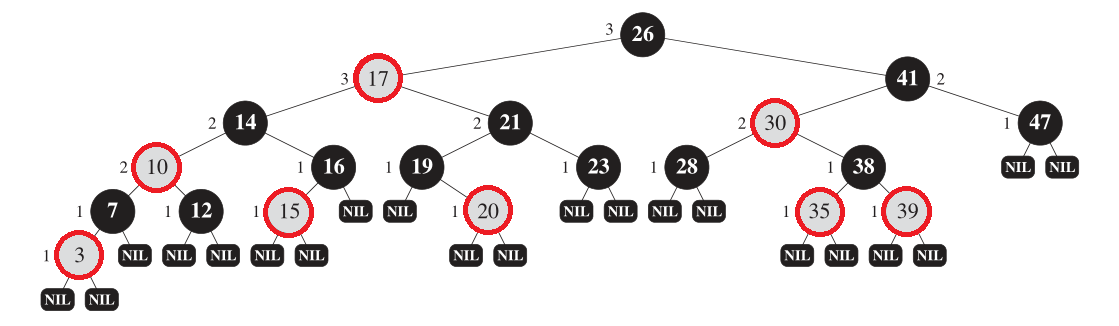
\includegraphics[width=7in]{assignment10-red-black-trees/original-tree.png}}
\caption{\label{fig:original-tree} A Sample Red-Black tree (Numbers next to nodes indicate their ``black height'')}
\end{figure}

\vspace{20pt}
{\bf Question (Insert nodes in the Red-Black Tree).}\\

\vspace{5pt}
{\bf (A)} Compute the following three key values ($u$, $v$, and $w$): 
$$\left\{ \begin{array}{l}
u = 3(a+b)+2\\
v = 3(b+c)+1\\
w = 3(c+a)\\ 
\end{array} \right.$$
Here $a,b,c$ are the last $3$ digits of your Student ID.

\vspace{5pt}
{\bf (B)} Show how the tree looks after the nodes $u$, $v$ and $w$ (in this order)
are inserted in the Red-Black Tree shown in Figure~\ref{fig:original-tree}.

If any of the values $u,v,w$ coincide with existing nodes, they 
should not be inserted. (Red-Black trees and BSTs in general can handle duplicates; but here
we assume that it stores a map/set with unique keys.)

{\em Note.} In order to get a partial credit 
it is suggested that you also show the intermediate steps (the
tree after inserting just $u$; then the tree after both $u$ and $v$ are inserted, 
then the final tree, where all $u,v,w$ are inserted). 

{\em Note.} Try to follow the red-black tree update operations (Goodrich2011 p.475-480) 
closely. And most importantly \textendash{} check that your inserts preserve 
all the invariants (BST order invariant and the $4$ properties of red-black trees).



\end{document}



